% =====================================================================
%  MATH3030 Project Report
%  Build:  latexmk          (uses .latexmkrc -> XeLaTeX + biber)
% =====================================================================
\documentclass[a4paper, 11pt]{article}

% --- 1. Packages that do things (maths, figures, refs) ---------------
% =====================================================================
%  preamble.tex - functional packages only.
%  Nothing here should change how the document *looks*; that belongs in
%  themes/. Keep this file the same when you switch themes.
% =====================================================================

% --- Maths ------------------------------------------------------------
\usepackage{amsmath, amssymb, amsthm}
\usepackage{mathtools}

% --- Figures & tables -------------------------------------------------
\usepackage{graphicx}
\graphicspath{{figures/}}
\usepackage{subcaption}   % side-by-side figures: \begin{subfigure}
\usepackage{booktabs}     % nice tables: \toprule \midrule \bottomrule
\usepackage{float}
\usepackage{comment}      % \begin{comment} ... \end{comment} to hide blocks

% --- Bibliography -----------------------------------------------------
\usepackage[style=authoryear, backend=biber, maxcitenames=2]{biblatex}
%  Use \textcite{turing1952} -> "Turing (1952)"
%      \parencite{turk1991}  -> "(Turk 1991)"

% --- Links & cross-references (load hyperref late, cleveref last) -----
\usepackage{hyperref}
\usepackage[capitalise, noabbrev]{cleveref}
%  Use \cref{eq:gray-scott} -> "Equation 1", \cref{fig:spots} -> "Figure 2"

% --- Equation numbering by section: (2.1), (2.2), ... ------------------
\numberwithin{equation}{section}

% --- Theorem-like environments ----------------------------------------
\theoremstyle{definition}
\newtheorem{definition}{Definition}[section]
\newtheorem{example}[definition]{Example}
\theoremstyle{plain}
\newtheorem{theorem}[definition]{Theorem}
\newtheorem{proposition}[definition]{Proposition}
\theoremstyle{remark}
\newtheorem*{remark}{Remark}

% --- Drafting helper: \todo{...} shows in red; disable before submitting
\usepackage{xcolor}
\newcommand{\todo}[1]{\textcolor{red}{[TODO: #1]}}
% \renewcommand{\todo}[1]{}   % <- uncomment to hide all TODOs


% --- 2. Notation shortcuts -------------------------------------------
% =====================================================================
%  macros.tex - notation shortcuts. Define a symbol once here so it is
%  consistent everywhere, and can be changed in one place.
% =====================================================================

\newcommand{\R}{\mathbb{R}}
\newcommand{\diff}{\mathop{}\!\mathrm{d}}          % upright d: \diff t
\newcommand{\pd}[2]{\frac{\partial #1}{\partial #2}} % \pd{u}{t}
\newcommand{\lap}{\nabla^2}                          % Laplacian
\newcommand{\Jac}{J}                                 % Jacobian matrix
\DeclareMathOperator{\tr}{tr}                        % trace
% \det already exists in LaTeX

% Gray-Scott parameters (change symbols here if you switch convention)
\newcommand{\GSF}{F}
\newcommand{\GSk}{k}
\newcommand{\Du}{D_u}
\newcommand{\Dv}{D_v}


% --- 3. THEME: everything about how the document LOOKS ----------------
%  To change the look, point this at a different file in themes/.
%    themes/basic.tex  - plain LaTeX defaults (current)
%    themes/serif.tex  - Georgia + tighter margins, like your project plan
% =====================================================================
%  themes/basic.tex - a plain, safe starting look.
%  A theme file controls ONLY appearance: page size/margins, fonts,
%  heading style, spacing, colours, header/footer.
%  To make a new theme: copy this file, edit it, and change the
%  \input{themes/...} line in main.tex.
% =====================================================================

% --- Page layout ------------------------------------------------------
\usepackage[margin=2.5cm]{geometry}

% --- Fonts ------------------------------------------------------------
%  Default Latin Modern (works with pdfLaTeX and XeLaTeX).

% --- Paragraphs: space between, no indent ------------------------------
\usepackage[skip=6pt plus 1pt]{parskip}

% --- Links: no coloured boxes ------------------------------------------
\hypersetup{
  colorlinks = true,
  linkcolor  = black,
  citecolor  = black,
  urlcolor   = blue!50!black,
}


% --- 4. Bibliography --------------------------------------------------
\addbibresource{references.bib}

% --- Title information -------------------------------------------------
\title{Nonlinear Dynamics in Computer Graphics:\\
       Reaction--Diffusion Systems in Procedural Generation}
\author{Ragav Srinivasan}
\date{\today}

\begin{document}

\maketitle

\begin{abstract}
	We start by ti
\end{abstract}

\section{Introduction}
\label{sec:introduction}
% Structure 
\subsection{Structure of this report}
% Describe each section in their own line:
\Cref{sec:background} gives the background on reaction--diffusion systems and the phenomena they
model. We then discuss a famous result of Alan Turing on reaction--diffusion systems, and finally
focus on a simple reaction--diffusion system called the Gray--Scott model.
\Cref{sec:simulations} is my original contribution: a stability analysis of the Gray--Scott model
and a numerical simulation of it.
\Cref{sec:conclusion} gives the conclusion and possible extensions of this project.
\section{Background}
\label{sec:background}



\subsection{Procedural Generation}
\label{sec:procedural}

Procedural generation is a broad set of techniques in computer graphics that is used to create visuals, such as pseudo-realistic textures, terrains and surfaces on the fly. Instead of an artist painting every surface or sculpting every mountain, a developer writes a short program controlled by a few parameters, and the computer produces the detail, often on the fly as the player explores. This makes it possible to build large, \emph{lifelike} landscapes with mountains, rivers and vegetation at very little cost in memory and artist time \parencite{lagae2010}.


Procedural generation is a broad set of techniques in computer graphics that is used to create visuals, such as pseudo-realistic textures, terrains and surfaces on the fly. It eliminates the need for an artists to manually prototype and create their own worlds, Instead, a deterministic function is used to produce the desired visuals, on the fly as the player explores. This makes it possible to build large, \emph{lifelike} landscapes with mountains, rivers and vegetation with little impact to memory. \parencite{lagae2010}.


% TODO: add a source for the Minecraft example, or remove it.
A well-known example is Minecraft, which uses procedural techniques to generate its worlds and cave systems.

Procedural generation is based on many algorithms. In this section we study one of the most widely used algorithms: \emph{Perlin Noise}.

\paragraph{Origin.}
% TODO: cite a source for the Tron / MAGI / Academy Award facts (e.g. Perlin's NYU biography page).
Ken Perlin devised his noise function after working on the visual effects for Disney's 1982 film \emph{Tron} at Mathematical Applications Group, Inc.\ (MAGI), and published it in 1985 \parencite{perlin1985}. His discovery of technique was so pivotal to the industry that it earned him an Academy Award for Technical Achievement, and still sees widespread in modern day films and video games. \parencite{lagae2010}.

\paragraph{How Perlin noise works.}
Consider one dimension first. At every integer $i$ we fix a random gradient (slope) $g_i$. For a point $x$ between $i$ and $i+1$, let $t = x - i \in [0,1]$. Each of the two neighbouring lattice points contributes a straight line through zero with its own slope, and the two lines are blended together:
\begin{equation}
	\label{eq:perlin-1d}
	\mathrm{noise}(x) = \bigl(1 - s(t)\bigr)\, g_i\, t \;+\; s(t)\, g_{i+1}\,(t - 1),
	\qquad
	s(t) = 6t^5 - 15t^4 + 10t^3 .
\end{equation}
The blending curve $s$ rises smoothly from $0$ to $1$, and its first and second derivatives vanish at $t = 0$ and $t = 1$, so neighbouring pieces join without visible creases \parencite{perlin2002}. Two properties follow directly from \cref{eq:perlin-1d}: the noise is zero at every integer, and its bumps all have roughly the same width, about one lattice cell (\cref{fig:perlin}a). In two dimensions the idea is the same: each corner $\mathbf{c}$ of a grid square carries a random unit vector $\mathbf{g}_{\mathbf{c}}$, the corner contributes $\mathbf{g}_{\mathbf{c}} \cdot (\mathbf{x} - \mathbf{c})$, and the four contributions are blended with $s$ in each direction (\cref{fig:perlin}b).

\paragraph{Building textures from noise.}
A single layer of noise is smooth but bland. Natural surfaces have detail at many scales, so copies of the noise at doubled frequency and halved amplitude are added together:
\begin{equation}
	\label{eq:fbm}
	\mathrm{fBm}(\mathbf{x}) = \sum_{j=0}^{n-1} \frac{1}{2^j}\, \mathrm{noise}\!\left(2^j \mathbf{x}\right),
\end{equation}
which is known as fractal Brownian motion (\cref{fig:perlin}c). Replacing $\mathrm{noise}$ by $\lvert \mathrm{noise} \rvert$ in \cref{eq:fbm} gives a ``turbulence'' function, and feeding it into a simple formula produces a material. Perlin's classic marble, for example, is $\sin\bigl(x_1 + \mathrm{turbulence}(\mathbf{x})\bigr)$ \parencite{perlin1985}

% 	\centering
% 	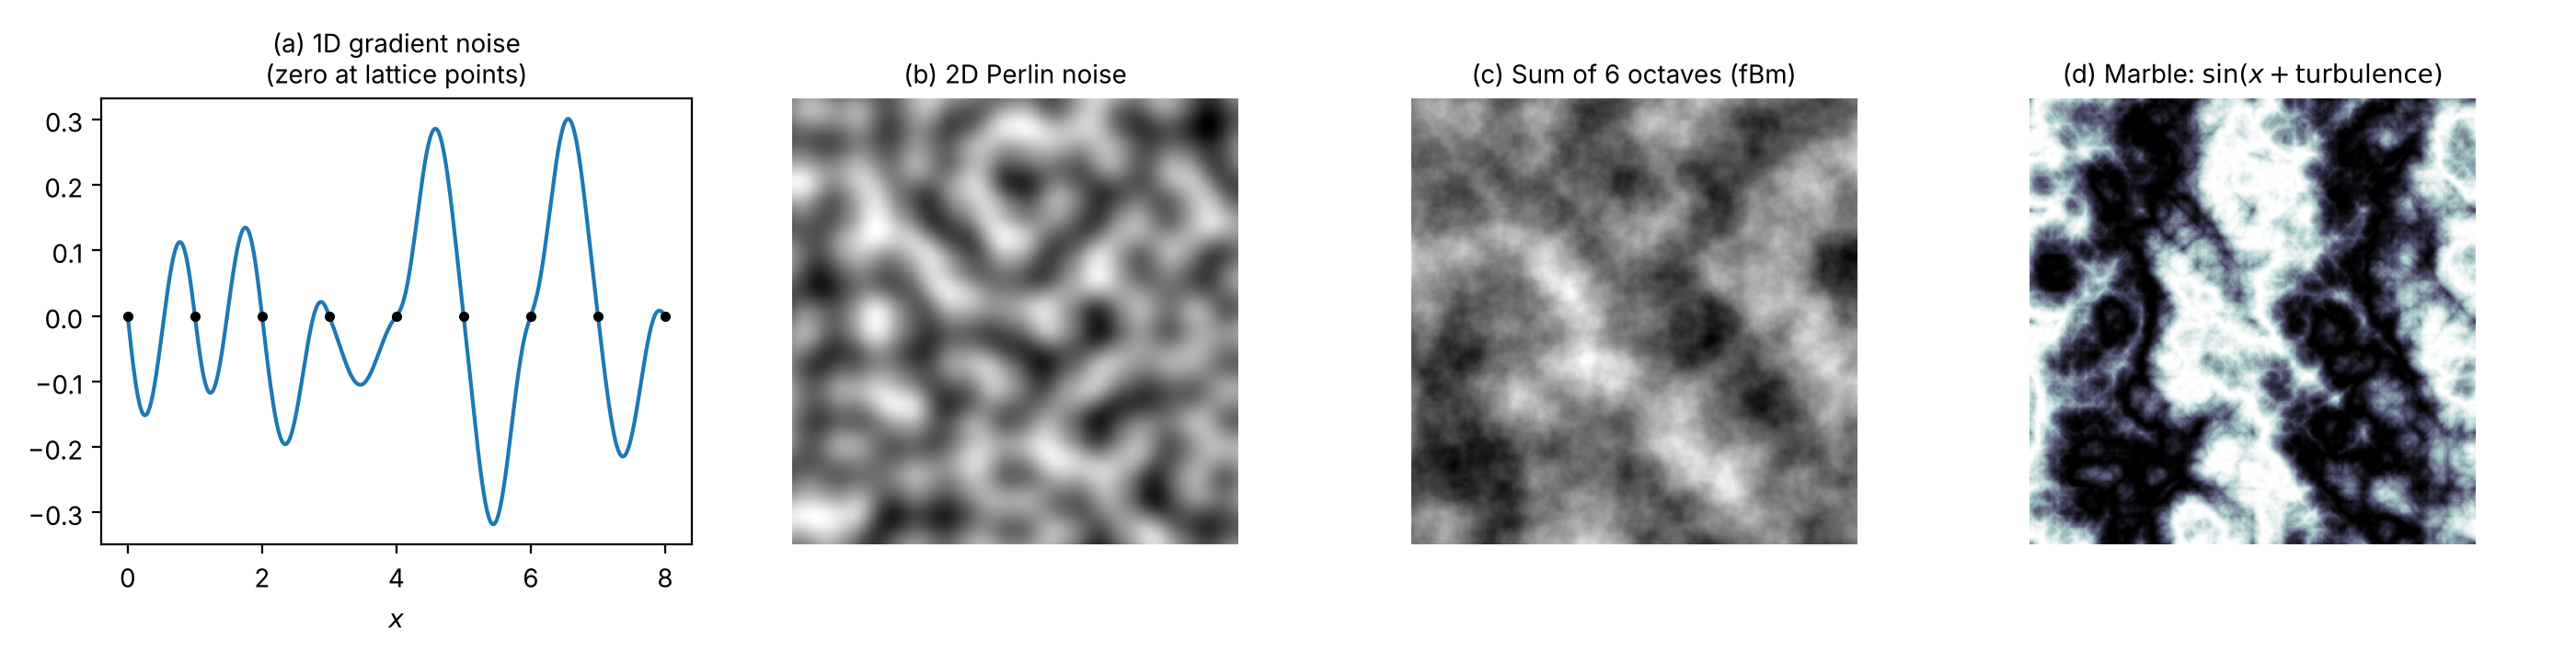
\includegraphics[width=\textwidth]{perlin_noise.png}
% 	\caption{Perlin noise, generated with our own implementation. (a) One-dimensional gradient noise, \cref{eq:perlin-1d}; it is zero at every lattice point (dots). (b) Two-dimensional Perlin noise. (c) Six octaves summed, \cref{eq:fbm}. (d) Marble, $\sin(x_1 + \mathrm{turbulence})$, after \textcite{perlin1985}.}
% 	\label{fig:perlin}
% \end{figure}

\paragraph{Limitations.}
Textures created with Perlin noise, and with noise functions in general, are random and have no organised structure \parencite{lagae2010}. Every bump has roughly the same size, but the bumps are placed at random: nothing makes spots evenly spaced or stripes run parallel. This is ideal for clouds, terrain or marble, but if we want a zebra whose stripes organise themselves, a different approach is needed. That approach is the subject of \cref{sec:rd-systems}.


\subsection{Reaction Diffusion Systems}
\label{sec:rd-systems}

% Segway to Reaction Diffusion Systems 

This brings us to the heart of this report, \emph{Reaction Diffusion Systems}. These are Nonlinear dynamical systems originating from the world of Chemistry that models the intereactions between multiple chemical susbtances and their diffusivity with resepct to space and time.
\\
\emph{Diffusion} refers to the spread of chemical substances between low and high concentration. It turns out adding an element of diffusion leads to some very interesting pattern formation.
\\
The General Form of Reaction Diffusion Systems is given by:

\begin{equation} \label{eq:rd-general}
	\pd{\mathbf{q}}{t} = D \nabla^2 \mathbf{q} + R(\mathbf{q}),
\end{equation}


% Explanation of the system
\begin{itemize}
	\item The equation is \emph{dimensionless}
	\item $\mathbf{q}$ is a vector of unknown vector functions representing the concentrations of an array of chemical substances.
	\item $D$ gives the diffusivity for each chemical
	\item $R(\mathbf{q}$) is another vector functions that describes all the chemical reactions.
\end{itemize}

There are several systems that fit the criteria of Reaction Diffusion Systems. Notably, the activator eqution, some russian equation, etc.


\subsection{Turing patterns}
\label{sec:turing-patterns}
\todo{Define Turing patterns} \\
Turing patterns are self organized patterns that resembles structures found in nature. \\
\todo{Cite turing's 1952 discovery on chemical morphogenesis}


\subsection{The Gray-Scott model}
\label{sec:gray-scott}

% Describes the problem
The setup for the Gray-Scott model supposes that we have a \emph{Well mixed tank} of chemical $U$. Then the concentration of $U$. We are interested in knowing the concentration of the chemical in space and time. For this, we define a vector function $u(x, t)$  that is currently unknown. We assume that chemical $U$ has the same concentration in the spatial domain except for a small patch in the center of the tank where chemical $V$ is introduced into the system. \\
\\
In chemistry, The relationship between $U$ and $V$ is defined as \textit{Autocatalysis} where the resulting product is a reactant, as is the case with $V$ is in the reaction shown below. The relationship is akin to that of \textit{prey and predator} models.

\begin{equation*}
	\underbrace{U + 2V \to 3V}_{\text{$V$ reacts to $U$ to make more of itself}}
	\qquad
	\underbrace{V \to P}_{\text{decay}}
\end{equation*}


The second rule suggests decay for $V$ by turning into an inert product $P$ which means that it becomes a non reactive substance.


% General form of the Gray Scott Model
\begin{align*}
	\frac{\partial U}{\partial t} & = -UV^2 + D_u \nabla^2 + f(1 - U) \\
	\frac{\partial V}{\partial t} & = UV^2 + D_v \nabla^2 + (k + f)V
\end{align*}
% Explaination of the terms 
\begin{itemize}
	\item $D_u$ and $D_v$ is the diffusivity of chemicals $U$ and $V$.
	\item $U$ and $V$ are the unknown vector functions representing the concentrations of the respective chemicals in space and time.
	\item $f$ is the feed rate of chemical $U$ for $V$
	\item $k$ is the decay rate for chemical $V$.
\end{itemize}

% What we are going to do with this model 
The broader goal of this project is to explain pattern formation rising from Reaction Diffusion Systems but the narrower goal is to find which parameter values of $F$ and $k$. Therefore, In the end we will build a parameter map of the Gray Scott Model that can identify which patterns we get.


\section{Original Contribution}
\label{sec:simulations}

\subsection{Stability analysis}
\label{sec:stability}


% Definition of Stability Analysis
A stability analysis gives us a guess on the behaviour of the system. For instance, a system is said to be stable if solutions move away from the equillibrium point, otherwise an unstable system is when solutions move away from the equillibrium point.


Nonlinear Dynamical Systems are hard to solve analytically.




% Why are we studying the stability analysis for the gray scott model
The point of this stability analysis is to show how adding a diffusion effect can destabilize a system. This is also called as Turing instability.

% How do we do a Stability Analysis:
In this case, we will be doing a stability analysis twice. The first part will prove the Gray Scott Model is stable when we drop diffusion. In the second part we will show that the Gray Scott Model's turing unstable after adding the diffusion constant.


%% Maths for Stability analysis 
1. Setup the Gray Scott system  as follows:
\begin{align*}
	\dot{U} = -UV^2 + D_u \nabla^2 + F(1 - U) \\
	\dot{V} = UV^2 + D_v \nabla^2 + (F + k)V
\end{align*}

2. What are the equillibrium points:
From inspection, there are two $(0, 0)$ and $(1, 0)$.

3. Jacobian of the gray-scott model:
\begin{align*}
	J = \begin{pmatrix}
		    \partial_{u} \dot{U} & \partial_v  \dot{U}  \\
		    \partial_{u} \dot{V} & \partial_{v} \dot{V}
	    \end{pmatrix}
	=
	\begin{pmatrix}
		- V^2 - F & -2UV     \\
		V^2       & (F + k)V
	\end{pmatrix}
\end{align*}

4. Substitute equillibrium points into jacobian

First equillibrium point:
\begin{align*}
	J(0, 0) = \begin{pmatrix}
		          -F & 0       \\
		          0  & (F + k)
	          \end{pmatrix}
\end{align*} \\

$p = Tr(J(0,0)) = k$  and  $q = \det(J(0,0)) = -F(F + k)$ \\
what is $p^2 - q$? \\
\todo{Write your stability analysis} Therefore, the system is \emph{stable}.



Substituting the second equillibrium point yields:
\begin{align*}
	J(1, 0) = \begin{pmatrix}
		          -F & 0 \\
		          0  & 0
	          \end{pmatrix}
\end{align*}
$Tr(J(1,0)) = -F$  and  $\det(J(1,0)) = 0$ \\
Therefore, the system is \emph{stable}.



Part 2: We do the same analysis with the diffusion terms added back?

1. Equillibrium points
2. Jacobian
3. Tr J and Det J of the jacobian
4. Is it stable or unstable.

\subsection{Simulation of the Gray Scott Model}
\label{sec:numerical}
% Movtiation for doing a numerical simulation
\subsection{Texture Mapping in Blender}
\todo{I will do this section if I have time, for now I will just do the parameter map and stability analysis.}



\todo{Method details, figures and discussion.}
\section{Conclusion}
\label{sec:conclusion}
\todo{Summarise what the stability analysis predicts, how well the simulation matches it, and what
	this means for someone choosing $F$ and $k$ to generate textures. Possible extensions: varying the
	diffusion ratio $D_u/D_v$, comparing the predicted and simulated spot spacing, and running the
	simulation on a 3D surface as in \textcite{turk1991}.}

\printbibliography


\section{Appendix}
\end{document}

